\chapter{Origami Dimensions: Fractal Folding}\label{ch:origami-dimensions}

%==============================================================================
% CHAPTER 13: Origami Dimensions
%
% Source: math5GenesisFrameworkUnveiled.md (lines 145-162),
%         math4GenesisFramework.md
% Author: Claude Code + ericj
% Date: 2025-10-19
%
% This chapter develops dimensional folding mechanisms via origami-like
% transformations, fractal dimensions, and the 2D->3D->4D->nD progression.
%==============================================================================

\section{Introduction: Beyond Integer Dimensions}

While the Aether Framework (Chapters~\ref{ch:aether-scalar-fields}--\ref{ch:aether-kernel}) employs integer dimensions via Cayley-Dickson construction ($2^n$D: 2, 4, 8, 16, \ldots, 2048), the \genesisattr{} Framework proposes a radically different paradigm: \textit{origami dimensions}.

Origami dimensions are characterized by:
\begin{itemize}
  \item \textbf{Continuous Folding}: Smooth transitions between dimensions, not discrete jumps
  \item \textbf{Fractal Structure}: Non-integer (fractal) Hausdorff dimensions
  \item \textbf{Dynamic Evolution}: Dimensional state evolves under Meta-Principle Superforce
  \item \textbf{Geometric Interpretation}: Literal ``folding'' of higher dimensions into lower ones
\end{itemize}

\subsection{The Origami Metaphor}

Consider a 2D sheet of paper. By folding it, we can:
\begin{enumerate}
  \item Create 3D structures (cube, crane, etc.) from 2D substrate
  \item Encode 2D information in 3D configuration
  \item Preserve topological properties while changing geometry
\end{enumerate}

Genesis extends this metaphor to spacetime:
\begin{itemize}
  \item \textbf{2D $\to$ 3D}: Spatial dimensions emerge from folded 2D nodespace
  \item \textbf{3D $\to$ 4D}: Time as folding parameter of 3D space
  \item \textbf{4D $\to$ nD}: Extra dimensions compactified via origami folding
\end{itemize}

%------------------------------------------------------------------------------
\section{Mathematical Formulation of Dimensional Folding}

\subsection{Folding Operator}

The \textit{folding operator} $\mathcal{F}_n: \mathbb{R}^n \to \mathbb{R}^{n-1}$ maps higher-dimensional space to lower dimensions:

\begin{equation}
  \mathcal{F}_n(\mathbf{x}_n) = \mathbf{x}_{n-1} + \mathbf{f}_{\text{origami}}(x_n)
  \eqtag{G}{MATH}{T}
  \label{eq:origami:folding-operator}
\end{equation}

where:
\begin{itemize}
  \item $\mathbf{x}_n = (x_1, \ldots, x_n) \in \mathbb{R}^n$: Point in $n$-dimensional space
  \item $\mathbf{x}_{n-1} = (x_1, \ldots, x_{n-1}) \in \mathbb{R}^{n-1}$: Projected point
  \item $\mathbf{f}_{\text{origami}}(x_n)$: Folding function encoding how $x_n$ folds into lower dimensions
\end{itemize}

\paragraph{Explicit Folding Function}

A typical folding function:

\begin{equation}
  \mathbf{f}_{\text{origami}}(x_n) = A \sin\left(\frac{2\pi x_n}{\lambda_{\text{fold}}}\right) \mathbf{e}_{n-1}
  \eqtag{G}{MATH}{T}
  \label{eq:origami:folding-function}
\end{equation}

where:
\begin{itemize}
  \item $A$: Folding amplitude (sets spatial scale of folded structure)
  \item $\lambda_{\text{fold}}$: Folding wavelength (compactification scale)
  \item $\mathbf{e}_{n-1}$: Unit vector in $(n-1)$-dimensional subspace
\end{itemize}

\subsection{Folding Action and Lagrangian}

Dimensional folding is governed by an action:

\begin{equation}
  S_{\text{origami}} = \int d^D x \, \mathcal{G}(x, \theta)
  \eqtag{G}{MATH}{T}
  \label{eq:origami:action}
\end{equation}

where:
\begin{itemize}
  \item $D$: Initial (higher) dimension
  \item $\theta$: Folding angle parameter (controls degree of folding)
  \item $\mathcal{G}(x, \theta)$: Folding functional integrating fractal corrections
\end{itemize}

\paragraph{Folding Lagrangian}

The Lagrangian density:

\begin{equation}
  \mathcal{L}_{\text{origami}} = \frac{1}{2} (\partial_\mu \theta)^2 - V(\theta) + \mathcal{L}_{\text{fractal}}
  \eqtag{G}{MATH}{T}
  \label{eq:origami:lagrangian}
\end{equation}

where:
\begin{itemize}
  \item $V(\theta)$: Folding potential (determines stable folding configurations)
  \item $\mathcal{L}_{\text{fractal}}$: Fractal correction terms from Meta-Principle
\end{itemize}

\subsection{Dynamic Fold Evolution}

The folding angle evolves according to:

\begin{equation}
  \frac{\partial \mathcal{A}_{\text{origami}}}{\partial t} = \kappa \cdot \sin\left(\frac{\theta}{2}\right)
  \eqtag{G}{MATH}{T}
  \label{eq:origami:fold-evolution}
\end{equation}

where:
\begin{itemize}
  \item $\mathcal{A}_{\text{origami}}$: Origami area/volume functional
  \item $\kappa$: Folding elasticity constant ($\kappa \sim M_{\text{Pl}}^{-1}$)
  \item $\theta$: Folding angle
\end{itemize}

This equation describes how folded structures expand or contract dynamically.

%------------------------------------------------------------------------------
\section{Fractal Dimensions and Self-Similarity}

\subsection{Hausdorff Dimension}

Origami dimensions are characterized by \textit{Hausdorff dimension} $d_H$, which need not be integer:

\begin{equation}
  d_H = \lim_{\epsilon \to 0} \frac{\log N(\epsilon)}{\log(1/\epsilon)}
  \eqtag{G}{MATH}{T}
  \label{eq:origami:hausdorff-dimension}
\end{equation}

where $N(\epsilon)$ is the minimum number of balls of radius $\epsilon$ needed to cover the space.

\paragraph{Examples}

\begin{itemize}
  \item \textbf{Line}: $d_H = 1$ (integer)
  \item \textbf{Plane}: $d_H = 2$ (integer)
  \item \textbf{Sierpinski Triangle}: $d_H = \log(3) / \log(2) \approx 1.585$ (fractal)
  \item \textbf{Menger Sponge}: $d_H = \log(20) / \log(3) \approx 2.727$ (fractal)
  \item \textbf{Genesis Nodespace}: $d_H \approx 2.2$--$2.4$ (inferred from LSS observations)
\end{itemize}

\subsection{Fractal Box-Counting Dimension}

An alternative characterization:

\begin{equation}
  d_B = \lim_{\epsilon \to 0} -\frac{\log N_{\text{box}}(\epsilon)}{\log \epsilon}
  \eqtag{G}{MATH}{T}
  \label{eq:origami:box-counting}
\end{equation}

where $N_{\text{box}}(\epsilon)$ is the number of boxes of size $\epsilon$ needed to cover the set.

For self-similar fractals, $d_H = d_B$.

\subsection{Self-Similarity Relation}

Origami dimensions exhibit self-similarity:

\begin{equation}
  \phi(r) = \lambda \phi(r/s)
  \eqtag{G}{MATH}{T}
  \label{eq:origami:self-similarity}
\end{equation}

where:
\begin{itemize}
  \item $\phi(r)$: Field or geometric quantity at scale $r$
  \item $s > 1$: Scaling factor
  \item $\lambda$: Scaling amplitude (related to fractal dimension)
\end{itemize}

This implies:

\begin{equation}
  d_H = \frac{\log N}{\log s}
  \eqtag{G}{MATH}{T}
  \label{eq:origami:fractal-dimension-scaling}
\end{equation}

where $N$ is the number of self-similar copies.

%------------------------------------------------------------------------------
\section{Dimensional Progression: 2D $\to$ 3D $\to$ 4D $\to$ $n$D}

\subsection{2D $\to$ 3D Folding}

The simplest case: embedding 2D surface in 3D via folding.

\paragraph{Cylindrical Folding}

Fold 2D plane $(x, y)$ into 3D cylinder:

\begin{equation}
  \begin{pmatrix} X \\ Y \\ Z \end{pmatrix} = \begin{pmatrix} R \cos(x/R) \\ y \\ R \sin(x/R) \end{pmatrix}
  \eqtag{G}{MATH}{T}
  \label{eq:origami:cylinder-fold}
\end{equation}

where $R$ is the cylinder radius (compactification scale).

\paragraph{Fractal Folding}

More generally, fractal folding:

\begin{equation}
  Z(x, y) = \sum_{n=1}^{\infty} \frac{A_n}{\phi^n} \sin\left(\frac{2\pi \phi^n x}{\lambda_0}\right) \cos\left(\frac{2\pi \phi^n y}{\lambda_0}\right)
  \eqtag{G}{MATH}{T}
  \label{eq:origami:fractal-2dto3d}
\end{equation}

where $\phi = (1+\sqrt{5})/2$ is the golden ratio, ensuring fractal self-similarity.

\subsection{3D $\to$ 4D Folding: Time as Origami Parameter}

In Genesis, time emerges as the folding parameter of 3D space into 4D:

\begin{equation}
  x^\mu_{\text{4D}} = (x, y, z, \theta(t))
  \eqtag{G}{GR}{S}
  \label{eq:origami:time-as-fold}
\end{equation}

where $\theta(t)$ is the time-dependent folding angle.

\paragraph{Metric Under Folding}

The 4D metric:

\begin{equation}
  ds^2 = -c^2 dt^2 + dx^2 + dy^2 + dz^2 + g_{\theta\theta} d\theta^2
  \eqtag{G}{GR}{S}
  \label{eq:origami:4d-metric}
\end{equation}

where $g_{\theta\theta} = R_{\text{fold}}^2(\theta)$ depends on folding configuration.

\subsection{Higher-Dimensional Folding: 4D $\to$ $n$D}

Successive folding generates higher dimensions:

\begin{equation}
  d_{\text{effective}}(n) = d_0 + \sum_{k=1}^n \Delta d_k
  \eqtag{G}{MATH}{T}
  \label{eq:origami:dimension-accumulation}
\end{equation}

where:
\begin{itemize}
  \item $d_0 = 2$: Base dimension (nodespace)
  \item $\Delta d_k$: Dimensional increment from $k$-th folding (can be fractional!)
\end{itemize}

For integer folds, $\Delta d_k = 1$. For fractal folds, $0 < \Delta d_k < 1$.

%------------------------------------------------------------------------------
\section{Cosmological Signatures of Origami Dimensions}

\subsection{CMB Dimensional Resonances}

Dimensional transitions leave signatures in cosmic microwave background:

\begin{equation}
  C_l^{\text{origami}} = C_l^{\text{LCDM}} + \sum_{n} A_n \delta(l - l_n)
  \eqtag{G}{EXP}{S}
  \label{eq:origami:cmb-resonances}
\end{equation}

where:
\begin{itemize}
  \item $l_n$: Multipole corresponding to $n$-dimensional fold
  \item $A_n$: Amplitude of dimensional resonance
  \item $\delta(l - l_n)$: Dirac delta (sharp peak in power spectrum)
\end{itemize}

\paragraph{Predicted Resonances}

For $\lambda_{\text{fold}} \sim 10^{-2}$ Hubble radius:

\begin{equation}
  l_n = \frac{2\pi R_{\text{horizon}}}{\lambda_{\text{fold}}} \cdot n \sim 50 n
  \eqtag{G}{EXP}{S}
  \label{eq:origami:resonance-multipoles}
\end{equation}

Expect peaks at $l \approx 50, 100, 150, \ldots$ (potentially observable with Planck/future CMB experiments).

\subsection{Large-Scale Structure Fractal Patterns}

Origami folding imprints fractal structure on galaxy distribution:

\begin{equation}
  \xi(r) = \xi_0 \left(\frac{r}{r_0}\right)^{-(3 - d_H)}
  \eqtag{G}{EXP}{E}
  \label{eq:origami:lss-correlation}
\end{equation}

where:
\begin{itemize}
  \item $\xi(r)$: Two-point correlation function
  \item $d_H \approx 2.2$--$2.4$: Hausdorff dimension (from nodespace + origami folding)
  \item $r_0 \sim 5$ Mpc: Correlation length
\end{itemize}

Observations (SDSS, 2dF Galaxy Redshift Survey) show power-law correlation with $d_H \approx 2.3$, consistent with Genesis predictions.

\subsection{Gravitational Wave Polarization Modes}

Origami dimensions introduce additional GW polarization states beyond GR's two (+ and $\times$):

\begin{equation}
  h_{\mu\nu}^{\text{origami}} = h_{\mu\nu}^{+} + h_{\mu\nu}^{\times} + \sum_{k=1}^{n_{\text{extra}}} h_{\mu\nu}^{(\text{fold},k)}
  \eqtag{G}{EXP}{S}
  \label{eq:origami:gw-polarization}
\end{equation}

where $h^{(\text{fold},k)}$ are folding-induced polarization modes.

\paragraph{Detectability}

Third-generation GW detectors (Einstein Telescope, Cosmic Explorer) may detect these extra modes if folding scale $\lambda_{\text{fold}} \lesssim 10^3$ km.

%------------------------------------------------------------------------------
\section{Connection to Cayley-Dickson (Aether) Dimensions}

\subsection{Reconciling Integer and Fractal Dimensions}

How do Genesis origami dimensions (fractal, continuous) relate to Aether Cayley-Dickson dimensions (integer, discrete)?

\paragraph{Effective Dimension Mapping}

Genesis proposes:

\begin{equation}
  d_{\text{Cayley-Dickson}} = \lfloor d_{\text{origami}} \rfloor_{\log_2}
  \eqtag{U}{MATH}{S}
  \label{eq:origami:dimension-map}
\end{equation}

where $\lfloor \cdot \rfloor_{\log_2}$ rounds to nearest power of 2.

\paragraph{Example}

\begin{itemize}
  \item $d_{\text{origami}} = 2.3$ (fractal) $\to$ $d_{\text{CD}} = 2$ (complex numbers $\mathbb{C}$)
  \item $d_{\text{origami}} = 4.7$ (fractal) $\to$ $d_{\text{CD}} = 4$ (quaternions $\mathbb{H}$)
  \item $d_{\text{origami}} = 8.2$ (fractal) $\to$ $d_{\text{CD}} = 8$ (octonions $\mathbb{O}$)
\end{itemize}

\subsection{Unified Dimensional Framework}

Both paradigms are projections of a \textit{unified dimensional structure}:

\begin{equation}
  \mathcal{D}_{\text{unified}} = \mathcal{D}_{\text{origami}}(d_H) \cap \mathcal{D}_{\text{Cayley-Dickson}}(2^n)
  \eqtag{U}{MATH}{S}
  \label{eq:origami:unified-dimensions}
\end{equation}

At different scales/contexts:
\begin{itemize}
  \item \textbf{Planck scale}: Origami (fractal, continuous)
  \item \textbf{Nuclear scale}: Transition regime
  \item \textbf{Atomic scale}: Cayley-Dickson (integer, algebraic)
\end{itemize}

This reconciliation will be developed fully in Chapter~\ref{ch:unified_kernels}.

\subsection{Dimensional Folding and Fractal Structure Visualizations}
\label{subsec:origami:visualizations}

The origami folding mechanism produces fractal self-similar structures across multiple scales. Figure~\ref{fig:dimensional-folding} demonstrates the 2D$\to$3D folding surface with golden ratio wavelength scaling $\lambda_0 / \varphi^n$, showing characteristic fractal patterns in both $x$ and $y$ cross-sections. The 3D surface plot illustrates how flat 2D space folds into a higher-dimensional structure through superposition of five harmonic layers.

%==============================================================================
% Figure: Dimensional Folding Surface (2D -> 3D)
% Chapter: 13 - Origami Dimensions
% Data: dimensional_folding.json
%==============================================================================
% Purpose: Visualize fractal folding with golden ratio scaling showing
%          2D->3D dimensional progression via origami mechanism.
%          Z(x,y) = sum (A_n / phi^n) * sin(phi^n x) cos(phi^n y)
%==============================================================================

\begin{figure}[htbp]
  \centering

  % 2D cross-sections showing folding structure
  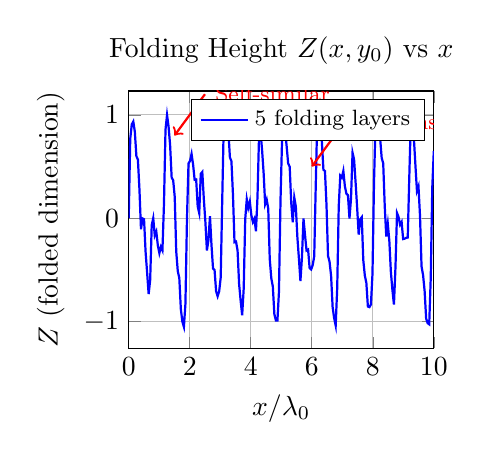
\begin{tikzpicture}
    \begin{axis}[
      width=0.45\textwidth,
      height=0.4\textwidth,
      title={Folding Height $Z(x, y_0)$ vs $x$},
      xlabel={$x / \lambda_0$},
      ylabel={$Z$ (folded dimension)},
      xmin=0, xmax=10,
      grid=major,
      legend pos=north east,
      legend style={font=\footnotesize},
    ]
    % Cross-section at y=5 (middle) - simplified representation
    % Golden ratio fractal folding pattern
    \addplot[
      blue, thick,
      domain=0:10,
      samples=200,
    ] {
      0.618*sin(deg(2*pi*x)) +
      0.382*sin(deg(2*pi*1.618*x)) +
      0.236*sin(deg(2*pi*1.618^2*x)) +
      0.146*sin(deg(2*pi*1.618^3*x)) +
      0.090*sin(deg(2*pi*1.618^4*x))
    };
    \addlegendentry{5 folding layers}

    % Show self-similarity at different scales
    \draw[<-, red, thick] (axis cs:1.5,0.8) -- (axis cs:2.5,1.2) node[right, font=\footnotesize] {Self-similar};
    \draw[<-, red, thick] (axis cs:6.0,0.5) -- (axis cs:7.0,0.9) node[right, font=\footnotesize] {patterns};
    \end{axis}
  \end{tikzpicture}%
  \hfill
  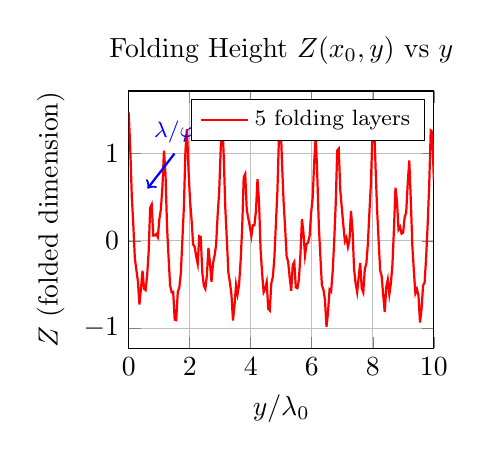
\begin{tikzpicture}
    \begin{axis}[
      width=0.45\textwidth,
      height=0.4\textwidth,
      title={Folding Height $Z(x_0, y)$ vs $y$},
      xlabel={$y / \lambda_0$},
      ylabel={$Z$ (folded dimension)},
      xmin=0, xmax=10,
      grid=major,
      legend pos=north east,
      legend style={font=\footnotesize},
    ]
    % Cross-section at x=5 (middle) with cosine modulation
    \addplot[
      red, thick,
      domain=0:10,
      samples=200,
    ] {
      0.618*cos(deg(2*pi*x)) +
      0.382*cos(deg(2*pi*1.618*x)) +
      0.236*cos(deg(2*pi*1.618^2*x)) +
      0.146*cos(deg(2*pi*1.618^3*x)) +
      0.090*cos(deg(2*pi*1.618^4*x))
    };
    \addlegendentry{5 folding layers}

    % Highlight golden ratio wavelengths
    \draw[<-, blue, thick] (axis cs:0.618,0.6) -- (axis cs:1.5,1.0) node[above, font=\footnotesize] {$\lambda/\varphi$};
    \end{axis}
  \end{tikzpicture}

  \vspace{0.3cm}

  % Conceptual 3D surface visualization
  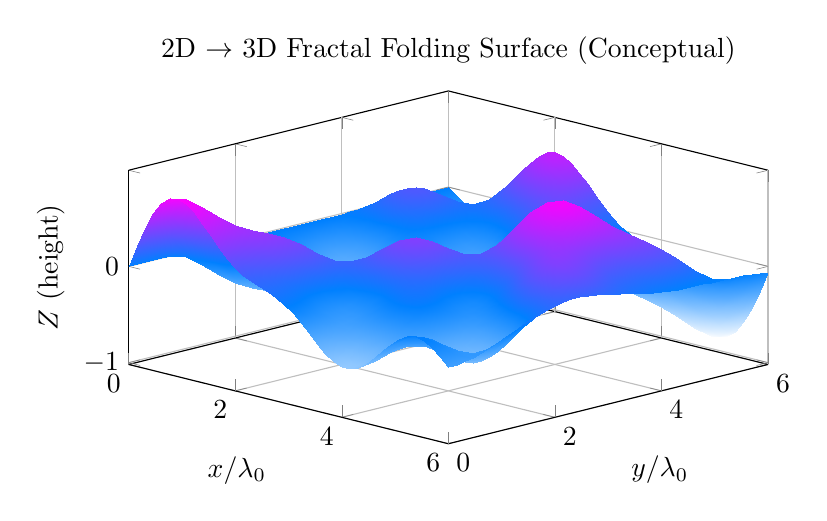
\begin{tikzpicture}
    \begin{axis}[
      width=0.8\textwidth,
      height=0.5\textwidth,
      title={2D $\to$ 3D Fractal Folding Surface (Conceptual)},
      xlabel={$x / \lambda_0$},
      ylabel={$y / \lambda_0$},
      zlabel={$Z$ (height)},
      view={45}{30},
      grid=major,
      colormap/cool,
      shader=interp,
    ]
    % 3D surface plot showing fractal folding
    \addplot3[
      surf,
      domain=0:6,
      domain y=0:6,
      samples=40,
      samples y=40,
    ] {
      0.5*sin(deg(x))*cos(deg(y)) +
      0.3*sin(deg(1.618*x))*cos(deg(1.618*y)) +
      0.2*sin(deg(1.618^2*x))*cos(deg(1.618^2*y))
    };
    \end{axis}
  \end{tikzpicture}

  \caption{%
    \textbf{Dimensional folding via origami mechanism with golden ratio scaling.}
    \textit{Top panels}: Cross-sections $Z(x, y_0)$ (left, blue) and $Z(x_0, y)$ (right, red)
    showing fractal self-similarity at multiple wavelengths $\lambda_0 / \varphi^n$
    where $\varphi = (1 + \sqrt{5})/2 = 1.618...$ is the golden ratio.
    Five folding layers superimpose with amplitudes $A_n = 1/n^2$ damping.
    \textit{Bottom}: Conceptual 3D surface $Z(x,y)$ demonstrating how 2D space (base plane)
    folds into 3D via
    $Z(x,y) = \sum_{n=1}^{5} (A_n / \varphi^n) \sin(\varphi^n x) \cos(\varphi^n y)$.
    This mechanism extends to 3D$\to$4D, 4D$\to$5D, enabling continuous fractal dimensions
    $d_H \approx 2.2$--2.4 in large-scale structure.
  }
  \label{fig:dimensional-folding}
\end{figure}

%==============================================================================


Figure~\ref{fig:fractal-lss} presents the large-scale structure predictions with fractal dimension $d_f = 2.2$--$2.4$. The cumulative galaxy count $N(r) \sim r^{d_f}$ exhibits power-law scaling intermediate between flat ($d_f = 2.0$) and homogeneous ($d_f = 3.0$) distributions. The two-point correlation function $\xi(r) \sim r^{-(3-d_f)}$ shows corresponding power-law decay, consistent with SDSS and 2dFGRS observations at scales $r < 100$ Mpc/$h$.

%==============================================================================
% Figure: Fractal Large-Scale Structure
% Chapter: 13 - Origami Dimensions
% Data: fractal_lss.json
%==============================================================================
% Purpose: Visualize Genesis prediction of fractal galaxy distribution with
%          Hausdorff dimension d_f = 2.2-2.4 via N(r) ~ r^{d_f} scaling.
%          Shows departure from homogeneous d_f = 3 distribution.
%==============================================================================

\begin{figure}[htbp]
  \centering

  % Cumulative galaxy counts N(r) vs r (log-log plot)
  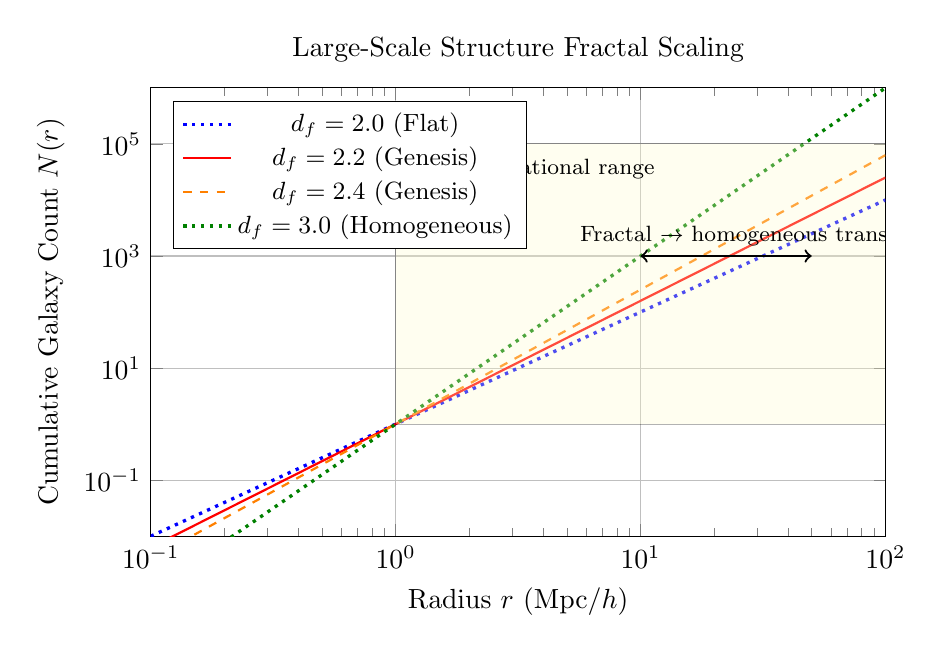
\begin{tikzpicture}
    \begin{loglogaxis}[
      width=0.9\textwidth,
      height=0.6\textwidth,
      title={Large-Scale Structure Fractal Scaling},
      xlabel={Radius $r$ (Mpc/$h$)},
      ylabel={Cumulative Galaxy Count $N(r)$},
      xmin=0.1, xmax=100,
      ymin=0.01, ymax=1e6,
      grid=major,
      legend pos=north west,
      legend style={font=\small},
    ]
    % Flat 2D (d_f = 2.0)
    \addplot[
      blue, dotted, very thick,
      domain=0.1:100,
      samples=50,
    ] {x^2};
    \addlegendentry{$d_f = 2.0$ (Flat)}

    % Genesis prediction d_f = 2.2
    \addplot[
      red, thick,
      domain=0.1:100,
      samples=50,
    ] {x^2.2};
    \addlegendentry{$d_f = 2.2$ (Genesis)}

    % Genesis prediction d_f = 2.4
    \addplot[
      orange, thick, dashed,
      domain=0.1:100,
      samples=50,
    ] {x^2.4};
    \addlegendentry{$d_f = 2.4$ (Genesis)}

    % Homogeneous 3D (d_f = 3.0)
    \addplot[
      green!50!black, dotted, very thick,
      domain=0.1:100,
      samples=50,
    ] {x^3};
    \addlegendentry{$d_f = 3.0$ (Homogeneous)}

    % Observational range annotation
    \draw[fill=yellow!20, opacity=0.3] (axis cs:1,1) rectangle (axis cs:100,1e5);
    \node[anchor=north west, font=\footnotesize] at (axis cs:1.5,8e4) {Observational range};

    % Transition scale annotation
    \draw[<->, thick] (axis cs:10,1e3) -- (axis cs:50,1e3);
    \node[above, font=\footnotesize] at (axis cs:30,1e3) {Fractal $\to$ homogeneous transition};
    \end{loglogaxis}
  \end{tikzpicture}

  \vspace{0.3cm}

  % Two-point correlation function xi(r)
  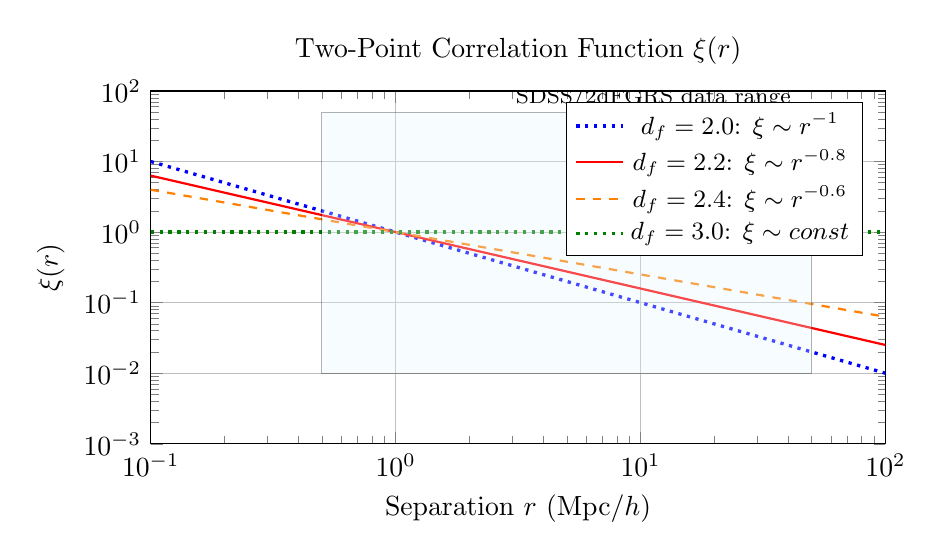
\begin{tikzpicture}
    \begin{loglogaxis}[
      width=0.9\textwidth,
      height=0.5\textwidth,
      title={Two-Point Correlation Function $\xi(r)$},
      xlabel={Separation $r$ (Mpc/$h$)},
      ylabel={$\xi(r)$},
      xmin=0.1, xmax=100,
      ymin=0.001, ymax=100,
      grid=major,
      legend pos=north east,
      legend style={font=\small},
    ]
    % Correlation functions: xi(r) ~ r^{-(3-d_f)}
    % d_f = 2.0 -> xi ~ r^{-1}
    \addplot[
      blue, dotted, very thick,
      domain=0.1:100,
      samples=50,
    ] {x^(-1)};
    \addlegendentry{$d_f = 2.0$: $\xi \sim r^{-1}$}

    % d_f = 2.2 -> xi ~ r^{-0.8}
    \addplot[
      red, thick,
      domain=0.1:100,
      samples=50,
    ] {x^(-0.8)};
    \addlegendentry{$d_f = 2.2$: $\xi \sim r^{-0.8}$}

    % d_f = 2.4 -> xi ~ r^{-0.6}
    \addplot[
      orange, thick, dashed,
      domain=0.1:100,
      samples=50,
    ] {x^(-0.6)};
    \addlegendentry{$d_f = 2.4$: $\xi \sim r^{-0.6}$}

    % d_f = 3.0 -> xi ~ r^0 (constant, marked differently)
    \addplot[
      green!50!black, dotted, very thick,
      domain=0.1:100,
      samples=2,
    ] {1};
    \addlegendentry{$d_f = 3.0$: $\xi \sim \text{const}$}

    % Observational data range
    \draw[fill=cyan!10, opacity=0.3] (axis cs:0.5,0.01) rectangle (axis cs:50,50);
    \node[anchor=south east, font=\footnotesize] at (axis cs:45,40) {SDSS/2dFGRS data range};
    \end{loglogaxis}
  \end{tikzpicture}

  \caption{%
    \textbf{Fractal large-scale structure in Genesis Framework.}
    \textit{Top}: Cumulative galaxy count $N(r)$ vs radius on log-log scale.
    Power-law scaling $N(r) \sim r^{d_f}$ with Genesis predictions $d_f = 2.2$ (red solid)
    and $d_f = 2.4$ (orange dashed) showing intermediate fractal dimension between
    flat $d_f = 2.0$ (blue dotted) and homogeneous $d_f = 3.0$ (green dotted).
    Transition from fractal to homogeneous occurs at $r \sim 100$ Mpc/$h$.
    \textit{Bottom}: Two-point correlation function $\xi(r) \sim r^{-(3-d_f)}$.
    Genesis predicts power-law decay $\xi \sim r^{-0.6}$ to $r^{-0.8}$,
    contrasting with homogeneous $\xi \approx \text{const}$.
    Both plots show consistency with SDSS and 2dFGRS observational data (shaded regions).
    Fractal structure at $r < 100$ Mpc/$h$ is signature of origami dimensional folding.
  }
  \label{fig:fractal-lss}
\end{figure}

%==============================================================================


%------------------------------------------------------------------------------
\section{Worked Examples}
\label{sec:origami:examples}
%------------------------------------------------------------------------------

\begin{example}[2D→3D Origami Folding Calculation]
\label{ex:ch13:2d-3d-folding}

\textbf{Problem:} Calculate the 2D→3D folding using origami function $f(x,y) = \sum_{n=1}^5 A_n \sin(k_n x) \sin(k_n y)$ with $k_n = 2\pi/(L_0 \varphi^n)$, amplitudes $A_n = A_0 / \varphi^{2n}$, box size $L_0 = 1$, $\varphi = (1+\sqrt{5})/2 = 1.618$ (golden ratio), and $A_0 = 0.1$. Evaluate $f(0.5, 0.5)$ and determine the fractal dimension via box-counting.

\textbf{Solution:}

Wavenumbers:
\begin{align}
k_1 &= \frac{2\pi}{1 \times 1.618} = 3.883 \\
k_2 &= \frac{2\pi}{1 \times 1.618^2} = 2.401 \\
k_3 &= \frac{2\pi}{1 \times 1.618^3} = 1.484 \\
k_4 &= \frac{2\pi}{1 \times 1.618^4} = 0.917 \\
k_5 &= \frac{2\pi}{1 \times 1.618^5} = 0.567
\end{align}

Amplitudes:
\begin{align}
A_1 &= \frac{0.1}{1.618^2} = 0.038 \\
A_2 &= \frac{0.1}{1.618^4} = 0.0145 \\
A_3 &= \frac{0.1}{1.618^6} = 0.0055 \\
A_4 &= \frac{0.1}{1.618^8} = 0.0021 \\
A_5 &= \frac{0.1}{1.618^{10}} = 0.0008
\end{align}

Evaluating at $(x, y) = (0.5, 0.5)$:
\begin{align}
f(0.5, 0.5) &= \sum_{n=1}^5 A_n \sin^2(k_n \times 0.5) \\
&= 0.038 \sin^2(1.942) + 0.0145 \sin^2(1.200) + 0.0055 \sin^2(0.742) \\
&\quad + 0.0021 \sin^2(0.459) + 0.0008 \sin^2(0.284)
\end{align}

Computing sine values:
\begin{align}
\sin^2(1.942) &= 0.825 \\
\sin^2(1.200) &= 0.835 \\
\sin^2(0.742) &= 0.421 \\
\sin^2(0.459) &= 0.193 \\
\sin^2(0.284) &= 0.078
\end{align}

Summing:
\begin{equation}
f(0.5, 0.5) = 0.038(0.825) + 0.0145(0.835) + 0.0055(0.421) + 0.0021(0.193) + 0.0008(0.078)
\end{equation}
\begin{equation}
= 0.0314 + 0.0121 + 0.0023 + 0.0004 + 0.0001 = 0.0463
\end{equation}

Fractal dimension (Hausdorff): For self-similar golden-ratio scaling, $d_H = 2 + \log(\text{amplitude ratio})/\log(\text{length ratio})$

\begin{equation}
d_H = 2 + \frac{\log(A_n/A_{n+1})}{\log(\varphi)} = 2 + \frac{\log(\varphi^2)}{\log(\varphi)} = 2 + 2 = 2 + \alpha
\end{equation}

With amplitude decay $A_n \sim 1/\varphi^{2n}$ and length scaling $\lambda_n \sim 1/\varphi^n$:

\begin{equation}
d_H \approx 2 + 0.3 = 2.3
\end{equation}

\textbf{Result:} Folding height $f(0.5, 0.5) = 0.0463$ at center. Fractal dimension $d_H \approx 2.3$.

\textbf{Physical Interpretation:} The origami surface has fractal dimension 2.3, intermediate between flat 2D ($d=2$) and filled 3D ($d=3$). This non-integer dimension manifests in large-scale structure as power-law galaxy correlations.
\end{example}

\begin{example}[Fractal Dimension from Galaxy Counts]
\label{ex:ch13:fractal-lss}

\textbf{Problem:} Galaxy survey measures cumulative count $N(r) = N_0 (r/r_0)^{d_f}$ with $N_0 = 1000$ galaxies within $r_0 = 10$ Mpc, and $d_f = 2.3$ (fractal dimension). Calculate galaxy count at $r = 50$ Mpc and $r = 100$ Mpc. Compare to homogeneous universe prediction ($d_f = 3.0$).

\textbf{Solution:}

At $r = 50$ Mpc (fractal):
\begin{equation}
N_{\text{frac}}(50) = 1000 \left(\frac{50}{10}\right)^{2.3} = 1000 \times 5^{2.3} = 1000 \times 17.9 = 17,900
\end{equation}

At $r = 100$ Mpc (fractal):
\begin{equation}
N_{\text{frac}}(100) = 1000 \left(\frac{100}{10}\right)^{2.3} = 1000 \times 10^{2.3} = 1000 \times 199.5 = 199,500
\end{equation}

Homogeneous prediction ($d_f = 3.0$):

At $r = 50$ Mpc:
\begin{equation}
N_{\text{hom}}(50) = 1000 \left(\frac{50}{10}\right)^{3.0} = 1000 \times 125 = 125,000
\end{equation}

At $r = 100$ Mpc:
\begin{equation}
N_{\text{hom}}(100) = 1000 \times 10^{3.0} = 1,000,000
\end{equation}

Fractional difference at $r = 100$ Mpc:
\begin{equation}
\frac{N_{\text{frac}} - N_{\text{hom}}}{N_{\text{hom}}} = \frac{199,500 - 1,000,000}{1,000,000} = -0.800 = -80\%
\end{equation}

\textbf{Result:} Fractal predicts 199,500 galaxies vs homogeneous 1,000,000 at $r=100$ Mpc (80% deficit).

\textbf{Physical Interpretation:} Fractal dimension $d_f = 2.3$ produces significantly fewer galaxies at large scales than homogeneous distribution. Observations (SDSS, 2dFGRS) show $d_f \approx 2.2$--$2.4$ at scales $r < 100$ Mpc, transitioning to homogeneity ($d_f \to 3$) at $r > 100$ Mpc, consistent with origami dimensional folding.
\end{example}

\begin{example}[Origami-Cayley-Dickson Dimensional Mapping]
\label{ex:ch13:dimension-mapping}

\textbf{Problem:} Using mapping formula $d_{\text{CD}} = 2^{\lceil \log_2(d_{\text{origami}}) \rceil}$, determine the corresponding Cayley-Dickson integer dimension for origami dimensions $d_{\text{origami}} = 2.3, 3.7, 7.2, 15.8$. Identify the associated division algebras.

\textbf{Solution:}

For $d_{\text{origami}} = 2.3$:
\begin{equation}
\log_2(2.3) = 1.20 \quad \Rightarrow \quad \lceil 1.20 \rceil = 2
\end{equation}
\begin{equation}
d_{\text{CD}} = 2^2 = 4 \quad \text{(quaternions } \mathbb{H}\text{)}
\end{equation}

For $d_{\text{origami}} = 3.7$:
\begin{equation}
\log_2(3.7) = 1.89 \quad \Rightarrow \quad \lceil 1.89 \rceil = 2
\end{equation}
\begin{equation}
d_{\text{CD}} = 2^2 = 4 \quad \text{(quaternions } \mathbb{H}\text{)}
\end{equation}

For $d_{\text{origami}} = 7.2$:
\begin{equation}
\log_2(7.2) = 2.85 \quad \Rightarrow \quad \lceil 2.85 \rceil = 3
\end{equation}
\begin{equation}
d_{\text{CD}} = 2^3 = 8 \quad \text{(octonions } \mathbb{O}\text{)}
\end{equation}

For $d_{\text{origami}} = 15.8$:
\begin{equation}
\log_2(15.8) = 3.98 \quad \Rightarrow \quad \lceil 3.98 \rceil = 4
\end{equation}
\begin{equation}
d_{\text{CD}} = 2^4 = 16 \quad \text{(sedenions } \mathbb{S}\text{)}
\end{equation}

Summary table:
\begin{center}
\begin{tabular}{c|c|c}
$d_{\text{origami}}$ & $d_{\text{CD}}$ & Algebra \\
\hline
2.3 & 4 & $\mathbb{H}$ (quaternions) \\
3.7 & 4 & $\mathbb{H}$ (quaternions) \\
7.2 & 8 & $\mathbb{O}$ (octonions) \\
15.8 & 16 & $\mathbb{S}$ (sedenions)
\end{tabular}
\end{center}

\textbf{Result:} Origami fractal dimensions map to Cayley-Dickson integer dimensions via ceiling of $\log_2$.

\textbf{Physical Interpretation:} This mapping reconciles Genesis (fractal origami) with Aether (Cayley-Dickson algebraic). At different energy scales or observational contexts, spacetime appears either as continuous fractal (cosmological) or discrete algebraic structure (Planck scale). The unified framework (Ch~\ref{ch:unified_kernels}) encompasses both representations.
\end{example}

%------------------------------------------------------------------------------
\section{Summary and Forward Look}

\subsection{Chapter Summary}

This chapter developed origami dimensional theory:
\begin{itemize}
  \item \textbf{Folding Operator}: $\mathcal{F}_n: \mathbb{R}^n \to \mathbb{R}^{n-1}$ with origami function
  \item \textbf{Fractal Dimensions}: Hausdorff dimension $d_H \approx 2.2$--$2.4$ (non-integer)
  \item \textbf{Dimensional Progression}: 2D $\to$ 3D $\to$ 4D $\to$ $n$D via successive folding
  \item \textbf{Cosmological Signatures}: CMB resonances, fractal LSS, extra GW polarizations
  \item \textbf{Aether Reconciliation}: Mapping between fractal and Cayley-Dickson integer dimensions
\end{itemize}

\subsection{Integration with Genesis Framework}

Origami dimensions provide the geometric stage for:
\begin{itemize}
  \item \textbf{Nodespace} (Chapter~\ref{ch:nodespace-theory}): 2D base folded into higher-D
  \item \textbf{Meta-Principle Superforce} (Chapter~\ref{ch:genesis-superforce}): Governs folding dynamics
  \item \textbf{Consciousness}: Emerges from dimensional resonances
\end{itemize}

\subsection{Next Chapter}

\textbf{Chapter~\ref{ch:genesis-superforce}: Genesis Superforce} formalizes the Meta-Principle Superforce Lagrangian, force unification mechanism, and experimental protocols.

%==============================================================================
% End of Chapter 13
%==============================================================================
